\documentclass[14pt]{extarticle}
\usepackage{amsmath}
\usepackage{amssymb}
%\usepackage{tikz}
%\usetikzlibrary{calc}
%\usetikzlibrary{trees}
\usepackage{hyperref}
\usepackage{graphicx}
\graphicspath{ {../../chap09/} }
\usepackage[top=0.75in, bottom=0.75in, left=0.75in, right=0.75in]{geometry}
%\newcommand*{\Scale}[2][4]{\scalebox{#1}{\ensuremath{#2}}}%
\usepackage[shortlabels]{enumitem}
\usepackage[most]{tcolorbox}
\definecolor{bg}{RGB}{255,249,227}
% \usepackage{showframe}
\title{\vspace{-5ex}Math 208 Section 9.7}
\date{\vspace{-10ex}}
%\usepackage{multicol}
%\setlength{\columnsep}{1cm}
\setlength{\parindent}{0pt}
\usepackage{parskip}
\setlength{\parskip}{10pt} % 1ex plus 0.5ex minus 0.2ex}
%\usepackage{ragged2e}


\begin{document}
	\maketitle		
	\section*{Homework, Reading, and Other}
	\begin{itemize}
		\item Section 9.5
		\item Section 9.7
	\end{itemize}

\section{Goals}
\begin{itemize}
	\item Recall and understand the business terminology
	\item Apply marginal analysis on costs revenues and profits
	\item Explain the results of your marginal analysis
\end{itemize}
		

\section{Section 9.7: Marginal Analysis}
In this section we will use the concepts of derivatives to application on some business problems. 

\subsection{Definitions}
In business, marginal cost is the instantaneous rate of change of cost relative to production at a given production level. In other words, the derivative.
\begin{center}
	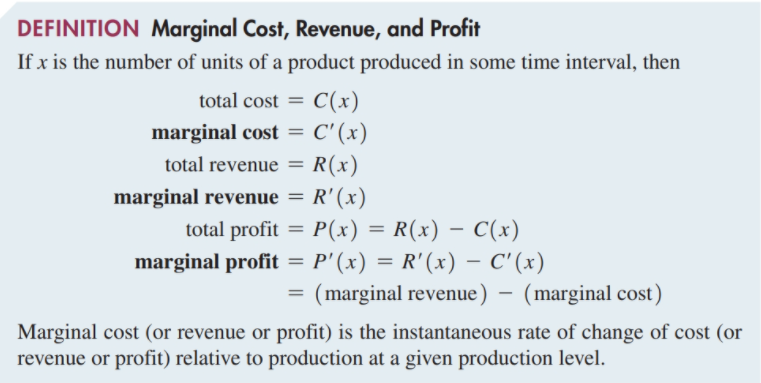
\includegraphics[width=0.9\linewidth]{9-7-1}
\end{center}
Where do these functions come from?
\begin{enumerate}
	\item Cost, $C(x)$, is usually given by the accounting department in coordination with operations.
	\item Demand of a product is typically given as a function of the price of the product. Know as the price-demand curve. We will often need to rearrange this equation. For example $x = 1000 - 100p$ becomes $p = 10-0.01x$.
	\item Revenue is equal to the price of a product times the number of units sold. $R(x)= xp$.
	\item Profit is revenues minus costs, $P(x) = R(x) - C(x)$.
\end{enumerate}
Often, you will be given the Cost function and the price-demand function. You will then need to rearrange the price-demand function and use that to determine the Revenue function. Now you can find the Price function.

\begin{tcolorbox}[enhanced jigsaw,colback=bg,boxrule=0pt,arc=0pt]
	\textbf{Exact Cost, Revenue, and Profit}
	\begin{align*}
		\text{exact cost} &= C(x+1)-C(x) \\
		\text{exact revenue} &= R(x+1) - R(x) \\
		\text{exact profit} &= P(x+1) - P(x)
	\end{align*}
\end{tcolorbox}
\begin{center}
	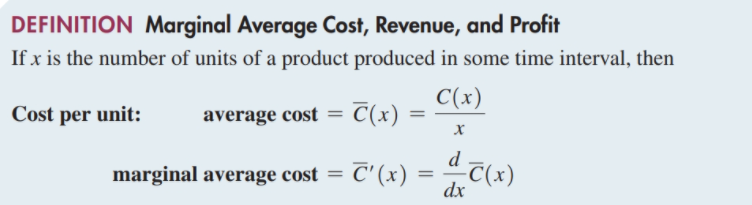
\includegraphics[width=0.9\linewidth]{9-7-2}
	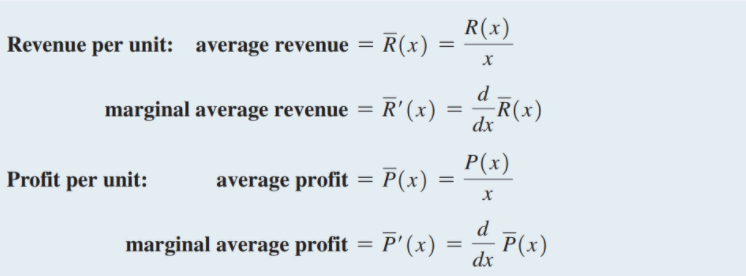
\includegraphics[width=0.9\linewidth]{9-7-3}
\end{center}



\subsection{Examples}
\subsubsection{Cost Analysis}
A company manufactures fuel tanks for cars. The total weekly cost (in dollars) of producing $x$ tanks is given by
$$C(x) = 10000+ 90x- 0.05x^2$$
\begin{enumerate}
	\item The marginal cost is $$C'(x)= 90-0.1x$$
	\item The marginal cost at a production level of 500 tanks is $$C'(500)= 90 -0.1(500) = \$40$$
	\item Interpretation is: At a production level of 500 tanks per week, the total production costs are increasing at the rate of \$40 per tank. So that the 501st tank should cost about \$40 to make.
	\item The exact cost of producing the 501st tank is. 
	\begin{align*}
		C(x+1)-C(x) &= C(501)-C(500) \\
		&= 10000 +90(501) - 0.05(501)^2 - 10000 + 90(500) - 0.05(500)^2 \\
		&= 42539.95 - 425000.00 \\
		&= \$39.95
	\end{align*} 
	You should notice that the marginal cost is approximately the exact cost but much easier to calculate. $C'(x) \approx C(x+1)-C(x)$.
\end{enumerate}

\subsubsection{Production Strategy}
A company’s market research department recommends the manufacture and marketing of a new headphone. The research department presents the following price-demand equation:
$$x = 10000-1000p$$

\begin{enumerate}
\item Where $x$ is the demand at price $p$. This price-demand equation will often need to be rearranged to give price as a function of demand, i.e.
$$p = 10 - 0.001x$$

\item Since both the price and the demand must be non-negative, we should verify the domain for $p$. When $x=0$, we note that $p>0$. Then
\begin{align*}
	p= 10 - 0.001x \geq 0 \\
	10 \geq 0.001x \\
	10,000 \geq 0
\end{align*}
Thus the domain is $0\leq x \leq 10,000$.

\item A company’s market research department recommends the manufacture and marketing of a new headphone. 

The finance department provides the cost function
$$C(x) = 7,000 + 2x $$
where \$7,000 is the estimate of fixed costs and \$2 is the estimate of variable costs per headphone.

This tells the marginal cost, that is $C'(x) = 2$.


\item Revenue is price times the number of units sold.
\begin{align*}
	R(x) &= xp = x(10 - 0.001x) \\
	& = 10x - 0.001x^2 \text{ for } 0\leq x \leq 10,000
\end{align*}

\item The marginal revenue is given by $$R'(x) = 10 - 0.002x$$
The marginal revenue at productions levels of $2000, 5000,$ and $7000$ is
\begin{align*}
	R'(2000) &= 6 \\
	R'(5000) &= 0 \\
	R'(7000) &= -4 
\end{align*}
The meaning of these numbers are not clear until we graph the Cost and Revenue functions and evaluate the Profit function.
\begin{center}
	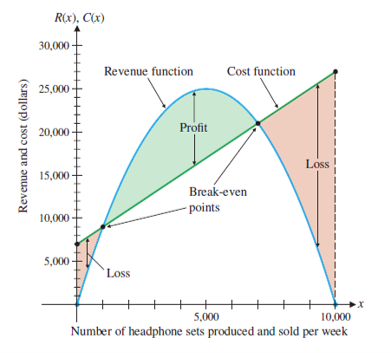
\includegraphics[width=0.7\linewidth]{9-7-20a}
\end{center}
Basically, we can see that revenue increases to create a profit and then reaches a maximum when $R'(x) = 0$. After this maximum, revenues start to decrease.

\item What is the profit function? $P(x) = R(x) - C(x)$. so that 
$$P(x) = 10x – 0.001x^2 – (7,000 + 2x) = –0.001x^2 + 8x – 7,000$$
\begin{center}
	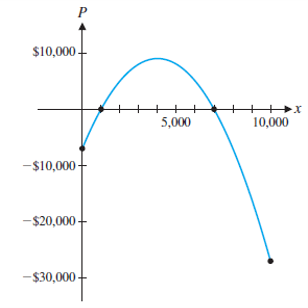
\includegraphics[width=0.5\linewidth]{9-7-20b}
\end{center}
You are making a profit on each unit sold when $1000 < x < 7000$.

\begin{tcolorbox}[enhanced jigsaw,colback=bg,boxrule=0pt,arc=0pt]
	\textbf{Caution:} This is not enough information to state either what price or what volume of production maximizes revenue. We will deal with this topic when we cover elasticity of demand in Chapter 10.
\end{tcolorbox}

\end{enumerate}

\subsubsection{Average Cost Analysis}
The total cost of printing $x$ dictionaries is
$$C(x) = 20,000+ 10x$$
\begin{enumerate}
	\item The average cost per unit if $x=1000$ dictionaries is $$\overline{C}(x) = \frac{C(x)}{x}= \frac{20000+10x}{x} = \frac{20,000}{x} + 10$$
	At a production level of $x=1000$, the average cost is
	$$\overline{C}(x)=\frac{20000}{1000} + 10 = 20,000x^{-1}+ 10 =\$30$$
	\item The marginal average cost at a production level of $x=1000$ is 
	$$\overline{C'}(x)= -\frac{20000}{x^2} $$
	$$ \overline{C'}(1000)=-\frac{20000}{1000^2}=-0.02$$
	This means that at $x=1000$ dictionaries, producing an additional dictionary reduces the cost per unit by $\$0.02$.
	\item What is the average cost per dictionary at $x=1001$? This would be the the average cost for at the 1000 production level plus the average marginal cost.
	$$\$30.00 + \$-0.02 = \$29.98$$
	\item In order to properly perform any Average Analysis, the average must be computed \textbf{prior} to the marginal average is computed.
\end{enumerate}





\noindent\rule{\textwidth}{1pt}
{\footnotesize Copyright (C) 2021 Garold Dalton --- Released under GNU General Public License v3.0}


\cleardoublepage


\end{document}
